\documentclass[a0,portrait]{a0poster}

\usepackage{multicol}

\usepackage[svgnames]{xcolor}
\usepackage[utf8]{inputenc}
\usepackage[german]{babel}
\usepackage[sfdefault]{ClearSans}
\usepackage{hyperref}
\usepackage{graphicx}
\usepackage[font=small,labelfont=bf]{caption}
\usepackage{booktabs}
\usepackage[font=small,labelfont=bf]{caption}
\usepackage{amsfonts, amsmath, amsthm, amssymb}
\usepackage{wrapfig}

\definecolor{fossgreen}{HTML}{14b967}
% remove column seperator
\setlength{\columnseprule}{0pt}
\columnsep=100pt

\begin{document}

\begin{minipage}[b]{0.75\linewidth}
\veryHuge \color{fossgreen} \textbf{Kunst, Creative Commons und Freie Software} \color{Black}\\\\
\huge \textbf{Free \& Open Source Software AG}\\[0.5cm]
\huge studentische Arbeitsgemeinschaft der TU Dortmund\\[0.4cm]
\Large \url{https://www.foss-ag.de}\\
\end{minipage}
\begin{minipage}[b]{0.25\linewidth}

\includegraphics[width=16cm]{figures/2000px.png}\\
\end{minipage}

\vspace{1cm}
\begin{multicols}{2}
\huge Egal ob Musikproduktion, Videoschnitt oder Bildbearbeitung, auch im kreativen Bereich gibt es eine große Auswahl an freier und quelloffener Software. Diese entsteht kollaborativ und ermöglicht es EntwicklernInnen aus ganzer Welt, daran mitzuwirken, um so eine stets besserwerdende Software zu schaffen, die der Allgemeinheit frei zur Verfügung steht. Freie Software ermöglicht es also jedem sich kreativ auszudrücken, ganz unabhängig der finanziellen Umstände. Dies ist insbesondere für SchülerInnen und Studierende interessant, die sich für Kunst interessieren oder sogar einen künstlerichen Studiengang belegen.\\\\
Einige Beispiele für solche freie Software-Alternativen sind das Bildbearbeitungsprogramm GIMP \footnote{\Large\url{https://www.gimp.org}}, das Audioschnittprogramm Audacity \footnote{\Large\url{https://www.audacityteam.org/}} oder die Animations und 3D-Design Software Blender \footnote{\Large\url{https://www.blender.org/}}.\\\\
Die auf dem Bildschirm gezeigten Filme (siehe rechte Spalte) wurden alle samt mit Blender erstellt und stehen unter einer Creative Commons Lizenz, die es der Allgemeinheit ermöglicht diese Filme nahezu uneingeschränkt zu nutzen. Somit ist nicht nur die Software, sondern auch die durch diese entstanden Werke als Gemeingut zu betrachten.

\columnbreak

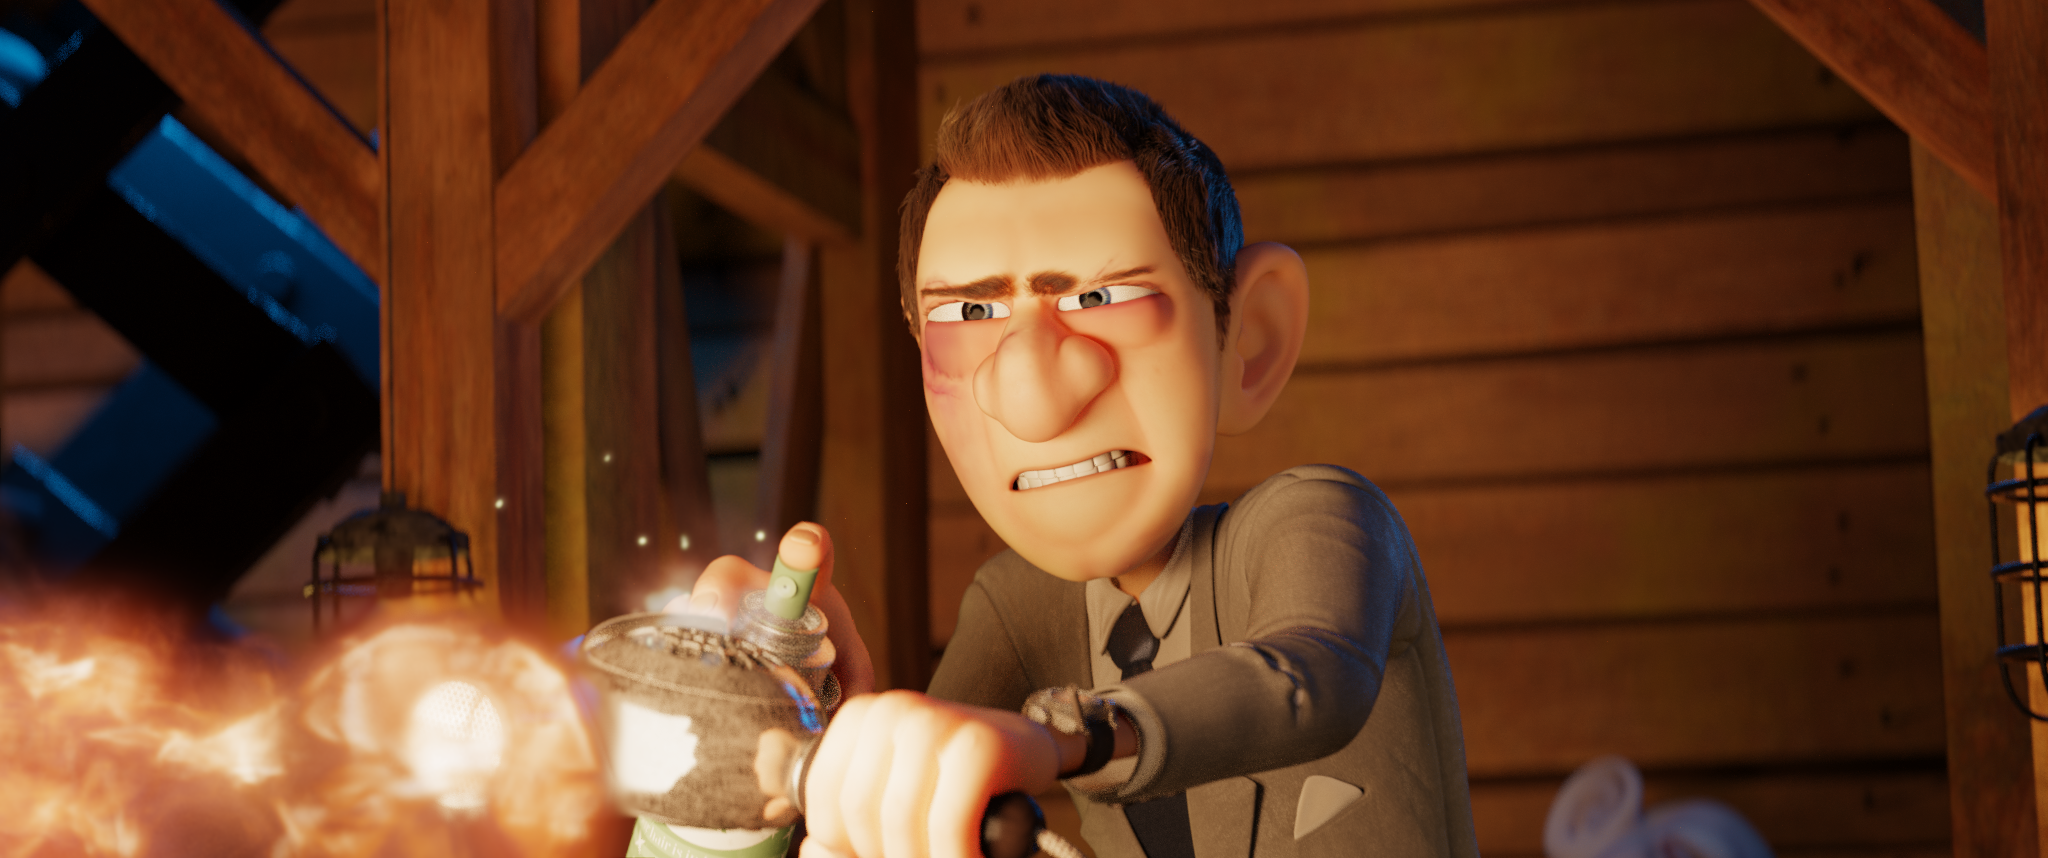
\includegraphics[scale=0.5]{figures/a327_barbershop_04861.png}
\captionof*{figure}{Agent 327 - Operation Barbershop (CC BY-ND)\\ \url{https://agent327.com/}}
\vspace*{2cm}

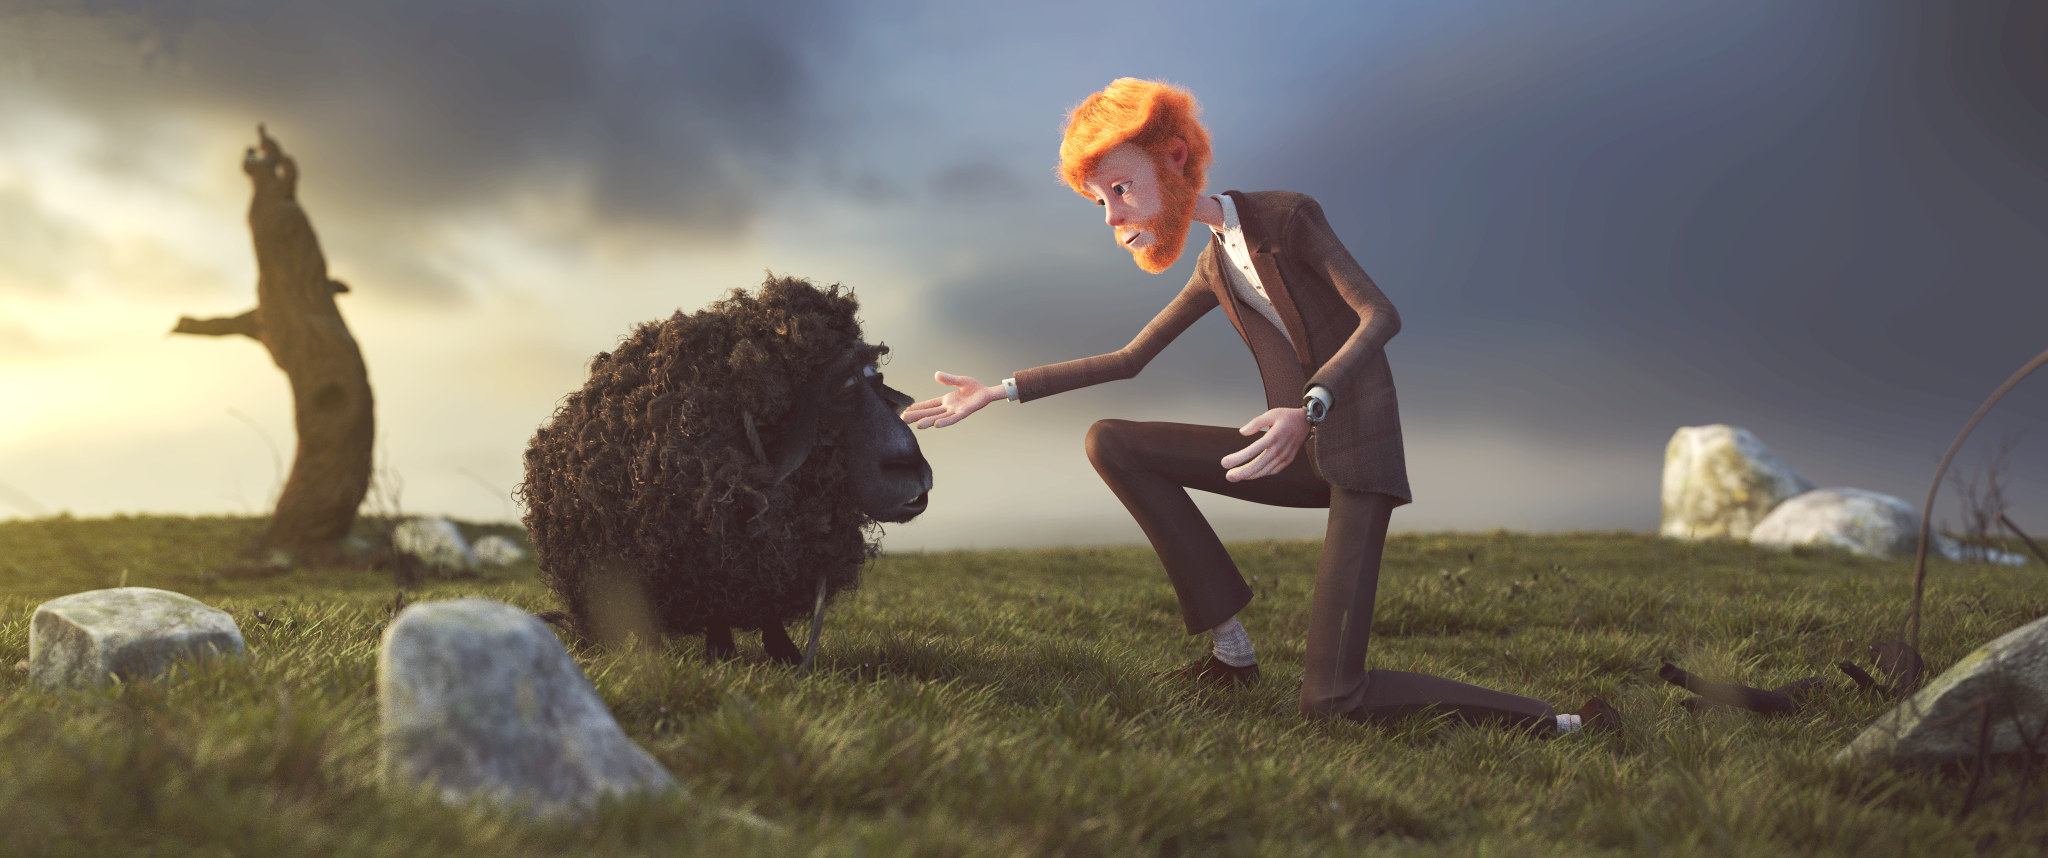
\includegraphics[scale=0.51]{figures/gooseberry_benchmark_01.jpg}
\captionof*{heading}{Cosmos Laundromat (CC BY 3.0)\\
\url{https://gooseberry.blender.org}}
\vspace*{2cm}


\includegraphics[scale=0.272]{figures/glasshalf.jpg}
\captionof*{figure}{Glass Half (CC BY)\\ 
\url{https://cloud.blender.org/p/glass-half/}}
\vspace*{2cm}

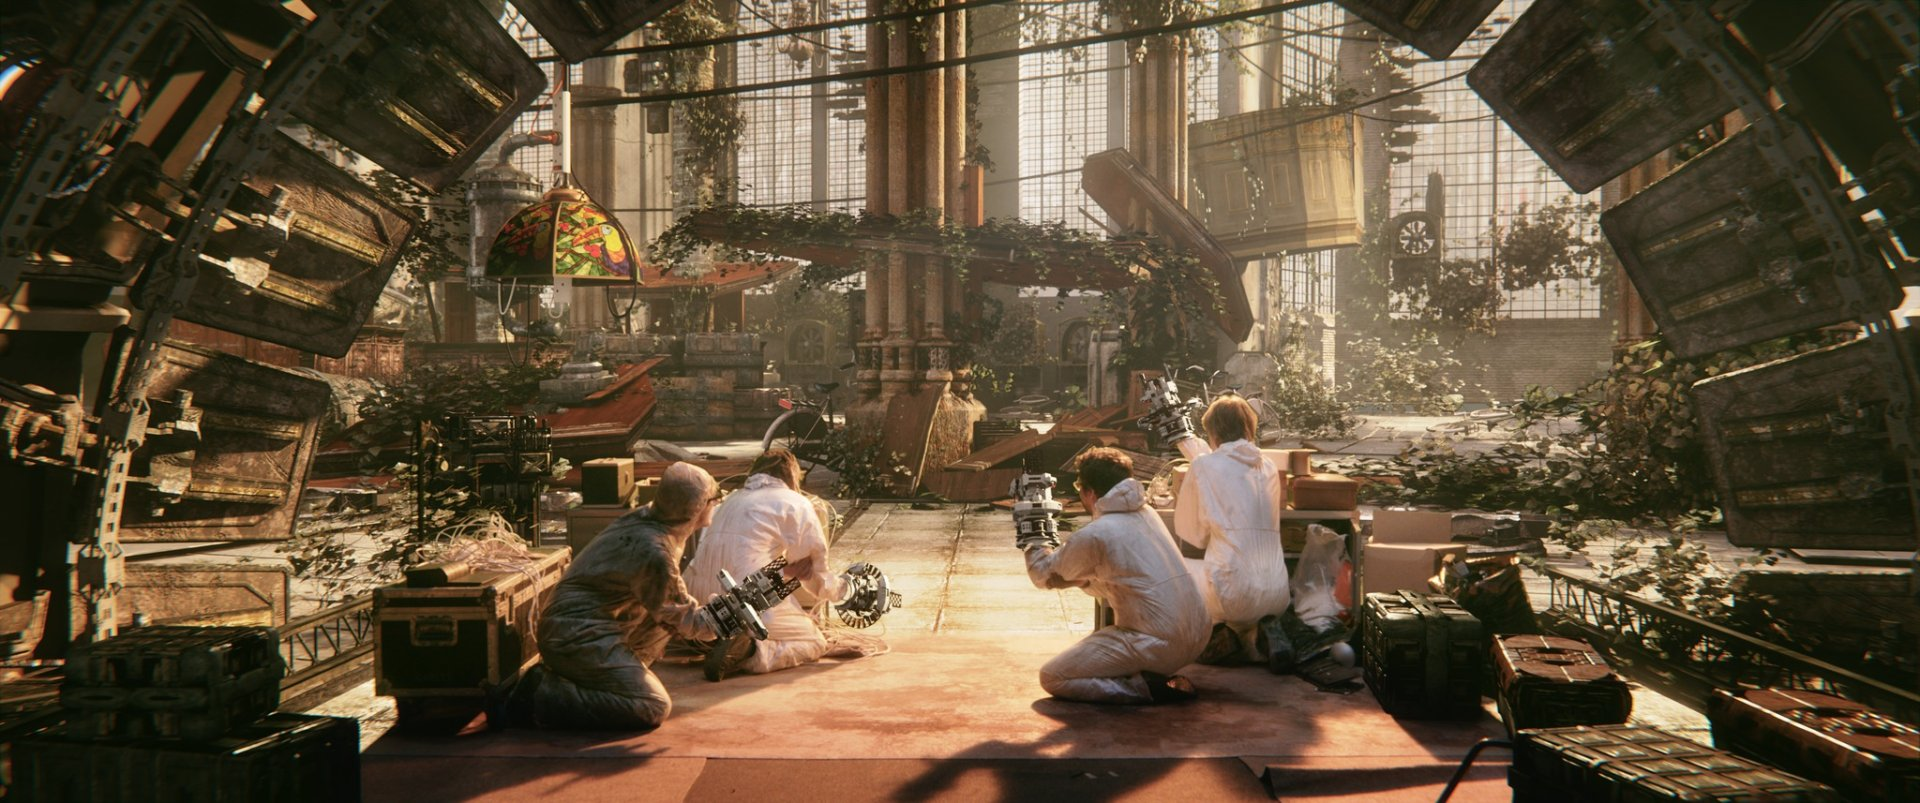
\includegraphics[scale=0.54]{figures/21_scientists_church.jpg}
\captionof*{figure}{Tears Of Steel (CC BY 3.0)\\
\url{https://mango.blender.org/}}
\end{multicols}
\end{document}